\documentclass{article}

\usepackage{tikz}
\usetikzlibrary{automata, positioning, arrows}

\usepackage{amsthm}
\usepackage{amsfonts}
\usepackage{amsmath}
\usepackage{amssymb}
\usepackage{fullpage}
\usepackage{color}
\usepackage{parskip}
\usepackage{hyperref}
  \hypersetup{
    colorlinks = true,
    urlcolor   = blue,   % color of external links
    linkcolor  = blue,   % color of internal links
    citecolor  = blue,   % color of links to bibliography
    filecolor  = blue    % color of file links
  }

\usepackage{listings}

\definecolor{dkgreen}{rgb}{0,0.6,0}
\definecolor{gray}{rgb}{0.5,0.5,0.5}
\definecolor{mauve}{rgb}{0.58,0,0.82}

\lstset{frame=tb,
  language=Python, % change to any language you prefer
  aboveskip=3mm,
  belowskip=3mm,
  showstringspaces=false,
  columns=flexible,
  basicstyle={\small\ttfamily},
  numbers=none,
  numberstyle=\tiny\color{gray},
  keywordstyle=\color{blue},
  commentstyle=\color{dkgreen},
  stringstyle=\color{mauve},
  breaklines=true,
  breakatwhitespace=true,
  tabsize=3
}

% ---------------------------------------------------------------------
% Theorem/Definition/Remark Environments
% ---------------------------------------------------------------------
\newtheoremstyle{theorem}
  {\topsep}   % ABOVESPACE
  {\topsep}   % BELOWSPACE
  {\itshape\/}  % BODYFONT
  {0pt}       % INDENT (empty value is the same as 0pt)
  {\bfseries} % HEADFONT
  {.}         % HEADPUNCT
  {5pt plus 1pt minus 1pt} % HEADSPACE
  {}          % CUSTOM-HEAD-SPEC

\theoremstyle{theorem} 
   \newtheorem{theorem}{Theorem}[section]
   \newtheorem{corollary}[theorem]{Corollary}
   \newtheorem{lemma}[theorem]{Lemma}
   \newtheorem{proposition}[theorem]{Proposition}

\theoremstyle{definition}
   \newtheorem{definition}[theorem]{Definition}
   \newtheorem{example}[theorem]{Example}

\theoremstyle{remark}    
  \newtheorem{remark}[theorem]{Remark}

\setcounter{tocdepth}{3}    % This makes subsubsections appear in TOC
\setcounter{secnumdepth}{3} % This makes subsubsections numbered

% ---------------------------------------------------------------------
% Title and Author
% ---------------------------------------------------------------------
\title{DFAs and NFAs}
\author{Max Randall \\ Chapman University}
\date{\today}

% ---------------------------------------------------------------------
% BEGIN DOCUMENT
% ---------------------------------------------------------------------
\begin{document}

\maketitle

\setcounter{tocdepth}{3}
\tableofcontents

% ---------------------------------------------------------------------
% Introduction
% ---------------------------------------------------------------------
\section{Introduction}\label{sec:intro}
In this report, we explore fundamental aspects of both deterministic and nondeterministic finite automata (DFAs and NFAs), including extended transition functions, product automaton construction for intersection, and state modifications for union. We further demonstrate the subset construction to establish the equivalence of NFAs and DFAs, showcasing the broad utility of these automata concepts in both theoretical and practical contexts.
\newpage
% ---------------------------------------------------------------------
% Week by Week (or Chapter by Chapter)
% ---------------------------------------------------------------------
\section{Exersizes}\label{sec:week-by-week}

\noindent
\subsection{Homework 1}\\
Let $\mathcal{A} = (Q, \Sigma, \delta: Q \times \Sigma \to Q, q_0, F)$ be a DFA. Explain in what way you can view $\mathcal{A}$ as an NFA by doing the following:
\begin{enumerate}
\item Let $\mathcal{A}$ denote the following DFA:

\[
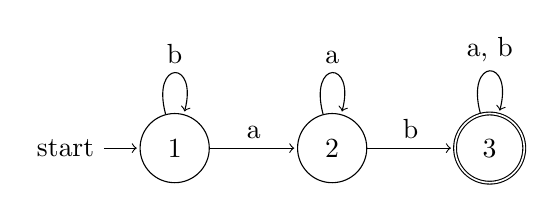
\begin{tikzpicture}[shorten >=1pt,node distance=2.0cm,on grid,auto]
   \node[state, initial] (q1) {1};
   \node[state] (q2) [right=of q1] {2};
   \node[state, accepting] (q3) [right=of q2] {3};

   \path[->]
   (q1) edge[loop above] node {b} (q1)
        edge node {a} (q2)
   (q2) edge[loop above] node {a} (q2)
        edge node {b} (q3)
   (q3) edge[loop above] node {a, b} (q3);
\end{tikzpicture}
\]

\noindent
Here:
\[
\begin{aligned}
Q &= \{1,2,3\}, \quad \Sigma = \{a,b\}, \\
q_0 &= 1, \quad F = \{3\}, \\
\delta(1,a) &= 2,\ \delta(1,b) = 1, \\
\delta(2,a) &= 2,\ \delta(2,b) = 3, \\
\delta(3,a) &= 3,\ \delta(3,b) = 3.
\end{aligned}
\]

Explain how you can understand $\mathcal{A}$ also as an NFA.
\item More generally, let $\mathcal{A} = (Q, \Sigma, \delta: Q \times \Sigma \to Q, q_0, F)$ be a DFA. Define an NFA
\[
\mathcal{A}' = (Q', \Sigma, \delta': Q' \times \Sigma \to \mathcal{P}(Q'), q_0', F')
\]
such that $L(\mathcal{A}) = L(\mathcal{A}')$.
\item Justify why your construction satisfies the desired condition.
\end{enumerate}

\subsection*{Solutions}

\subsubsection*{1) Viewing the Example DFA as an NFA}

A deterministic finite automaton (DFA) can be seen as a special case of a nondeterministic finite automaton (NFA) by interpreting its transition function in the following way: in an NFA, the transition function 
\[
\delta': Q \times \Sigma \to \mathcal{P}(Q)
\]
produces \emph{sets} of possible next states. In a DFA, however, for each state $q$ and input symbol $a$, there is exactly one next state $\delta(q,a)$. To view the DFA as an NFA, we simply set:
\[
\delta'(q,a) \;=\; \{\delta(q,a)\}.
\]
Hence, each transition in the original DFA becomes a transition to a \emph{singleton set} in the NFA. This preserves the language recognized, because in the NFA there is exactly one possible way to move from one state to another on a given symbol (i.e., no extra nondeterminism is introduced).

Concretely, for the illustrated DFA with states $1,2,3$, we define the NFA with the same states, same start state, same accepting states, and 
\[
\delta'(q,a) = \{\delta(q,a)\}\quad\text{and}\quad
\delta'(q,b) = \{\delta(q,b)\}.
\]

\subsubsection*{2) General Construction from a DFA to an NFA}

Given any DFA 
\[
\mathcal{A} = (Q, \Sigma, \delta, q_0, F),
\]
we can define an NFA
\[
\mathcal{A}' = (Q', \Sigma, \delta', q_0', F')
\]
as follows:
\begin{itemize}
\item $Q' = Q$ (we use exactly the same set of states),
\item $q_0' = q_0$ (same start state),
\item $F' = F$ (same set of accepting states),
\item For each $q \in Q$ and $a \in \Sigma$, set $\delta'(q,a) = \{\delta(q,a)\}$. 
\end{itemize}
Thus,
\[
\delta': Q' \times \Sigma \;\to\; \mathcal{P}(Q'), 
\quad
\delta'(q,a) = \bigl\{\delta(q,a)\bigr\}.
\]

\subsubsection*{3) Why $L(\mathcal{A}) = L(\mathcal{A}')$?}

The language recognized by a DFA is determined by the unique run from $q_0$ on any input string. In the constructed NFA, there is still exactly one possible transition at each step (the singleton set). So:
\begin{itemize}
\item If a string $w$ is accepted by the original DFA $\mathcal{A}$, then following the same path in $\mathcal{A}'$ is not only possible but is in fact the \emph{only} path. Thus $w$ is also accepted by $\mathcal{A}'$.
\item If a string $w$ is not accepted by the original DFA, then there is no way to reach an accepting state via $\delta$; hence in the NFA $\delta'$, which mimics these transitions in singleton sets, there is equally no path that leads to an accepting state.
\end{itemize}
Therefore, the two automata accept exactly the same set of strings, i.e., $L(\mathcal{A}) = L(\mathcal{A}')$.

\subsection{Homework 2}\\

\begin{enumerate}

\item Describe in words the language $L(A)$ accepted by the NFA $\mathcal{A}$ pictured below.


\item Specify the automaton $\mathcal{A}$ formally in the tuple form 
\[
(Q, \Sigma, \delta, q_0, F).
\]

\item Using the extended transition function $\hat{\delta}$ of $\mathcal{A}$, compute the set of states 
\[
\hat{\delta}(q_0,\,10110)
\]
step by step.

\item Find \emph{all} paths in $\mathcal{A}$ for the words $v = 1100$ and $w = 1010$. Represent each set of paths in a common diagram.

\item Construct the determinization $\mathcal{A}^D$ (the ``power set automaton'') of $\mathcal{A}$.

\item Verify that $L(\mathcal{A}) = L(\mathcal{A}^D)$.  Is there a smaller DFA that accepts the same language?

\end{enumerate}

\bigskip
\hrule
\bigskip

\subsection*{Solutions}

Below is the NFA $\mathcal{A}$:

\begin{center}
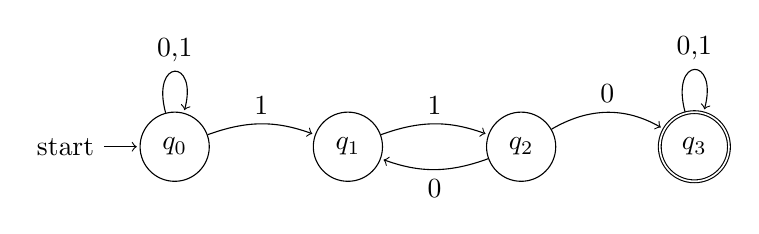
\begin{tikzpicture}[shorten >=1pt,node distance=2.2cm,on grid,auto]
   \node[state, initial] (q0) {$q_0$};
   \node[state] (q1) [right=of q0] {$q_1$};
   \node[state] (q2) [right=of q1] {$q_2$};
   \node[state, accepting] (q3) [right=of q2] {$q_3$};

   \path[->]
   (q0) edge[loop above] node {0,1} (q0)
        edge[bend left=20] node {1} (q1)
   (q1) edge[bend left=20] node {1} (q2)
   (q2) edge[bend left=20] node {0} (q1)
        edge[bend left=30] node {0} (q3)
   (q3) edge[loop above] node {0,1} (q3);
\end{tikzpicture}
\end{center}

\subsubsection*{1) Language Description}
Intuitively, the automaton $\mathcal{A}$ accepts exactly those binary strings for which there is a path from $q_0$ to the accepting state $q_3$.  
\begin{itemize}
\item A necessary part of reaching $q_3$ is taking the transition $q_2 \xrightarrow{0} q_3$. 
\item To get to $q_2$ in the first place, we must have used $q_1 \xrightarrow{1} q_2$. 
\item And to get to $q_1$, we must have used $q_0 \xrightarrow{1} q_1$ on some occurrence of the symbol 1 (rather than looping back to $q_0$ on that same~1).
\end{itemize}
Hence there must be at least two consecutive 1's used \emph{as the path} $q_0 \to q_1 \to q_2$, and then at least one 0 from $q_2$ to $q_3$.  Because $q_0$ loops on $\{0,1\}$, those symbols can appear arbitrarily often before the transition $q_0\to q_1$ is finally taken on a 1.  And from $q_2$, we can read a 0 that returns us to $q_1$ (followed by a 1 that goes back to $q_2$), repeatedly.  Eventually, a 0 from $q_2$ must go to $q_3$, after which any further symbols are accepted by the loop in $q_3$.  

In simpler terms: $\mathcal{A}$ accepts all binary strings that, \emph{on some nondeterministic choice of transitions}, contain two consecutive 1's used specifically to go from $q_0$ to $q_1$ to $q_2$, and eventually at least one 0 from $q_2$ to $q_3$.  After that point, the rest of the string can be anything.  

\subsubsection*{2) Formal NFA Specification }
We specify $\mathcal{A}$ as:
\[
\mathcal{A} \;=\; (\,Q,\;\Sigma,\;\delta,\;q_0,\;F\,),
\]
where:
\[
\begin{aligned}
Q &= \{\,q_0,q_1,q_2,q_3\},\\
\Sigma &= \{\,0,1\},\\
q_0 &= q_0 \text{ (the start state)},\\
F &= \{\,q_3\},\\
\delta(q_0,0) &= \{\,q_0\},\quad \delta(q_0,1) \;=\; \{\,q_0,\;q_1\},\\
\delta(q_1,0) &= \varnothing,\quad \delta(q_1,1) \;=\; \{\,q_2\},\\
\delta(q_2,0) &= \{\,q_1,\;q_3\},\quad \delta(q_2,1) \;=\; \varnothing,\\
\delta(q_3,0) &= \{\,q_3\},\quad \delta(q_3,1) \;=\; \{\,q_3\}.
\end{aligned}
\]

\newpage

\subsubsection*{3) Extended Transition Function on 10110}
Recall that the extended transition function $\hat{\delta}(r,x)$ for a state $r$ and input string $x$ returns \emph{all} possible states reachable from $r$ by reading $x$.  We compute 
\[
\hat{\delta}(q_0,\,10110)
\]
symbol by symbol:
\[
\begin{aligned}
\hat{\delta}(q_0,\epsilon) &= \{\,q_0\},\\
\hat{\delta}(q_0,1) &= \delta(q_0,1) = \{\,q_0,q_1\},\\
\hat{\delta}(\{q_0,q_1\},0) 
  &= \delta(q_0,0)\;\cup\;\delta(q_1,0) 
  = \{\,q_0\}\;\cup\;\varnothing 
  = \{\,q_0\},\\
\hat{\delta}(\{q_0\},1)
  &= \delta(q_0,1) 
  = \{\,q_0,q_1\},\\
\hat{\delta}(\{q_0,q_1\},1)
  &= \delta(q_0,1) \;\cup\;\delta(q_1,1) 
  = \{\,q_0,q_1\}\;\cup\;\{\,q_2\} 
  = \{\,q_0,q_1,q_2\}.
\end{aligned}
\]
Thus after reading \texttt{10110}, the set of possible states is $\{\,q_0,q_1,q_2\}$.  
(Note: if we continued with another symbol, we would then look at transitions from each state in $\{q_0,q_1,q_2\}$ on that symbol.)

\subsubsection*{4) All Paths for \texttt{v=1100} and \texttt{w=1010}}

\paragraph{All paths for \texttt{1100}.}
Starting in $q_0$ and reading \texttt{1100} step by step:
\[
\begin{aligned}
&\text{From }q_0\text{ on first `1':}\\
&\quad q_0 \;\xrightarrow{1}\; q_0 \quad\text{or}\quad q_0 \;\xrightarrow{1}\; q_1.\\[6pt]
&\text{Then on second `1':}\\
&\quad \text{if the first transition stayed in }q_0\text{, we again have }q_0 \;\xrightarrow{1}\; \{q_0,q_1\},\\
&\quad \text{if the first transition went to }q_1\text{, we must go }q_1 \;\xrightarrow{1}\; q_2.\\[6pt]
&\text{Then on first `0':}\\
&\quad \dots 
\end{aligned}
\]
One can systematically draw out the branching paths.  Eventually, any path that leads to $q_3$ must include the sub-path 
\[
q_0 \xrightarrow{1} q_1 \xrightarrow{1} q_2 \xrightarrow{0} q_3
\]
at some stage.

\paragraph{All paths for \texttt{1010}.}
A similar analysis shows that from $q_0$ on `1' we can stay in $q_0$ or move to $q_1$.  Then reading `0', etc.  You can depict these paths in a common diagram with branches for each nondeterministic choice.

\newpage

\subsubsection*{5) Determinization via Power Set Construction}
Define $\mathcal{A}^D = (Q^D,\,\Sigma,\,\delta^D,\,q_0^D,\,F^D)$ by:
\[
\begin{aligned}
Q^D &= \mathcal{P}(Q) = \{\varnothing,\;\{q_0\},\;\{q_1\},\;\dots,\;\{q_0,q_1\},\;\dots,\;\{q_0,q_1,q_2,q_3\},\dots\},\\
q_0^D &= \{q_0\},\\
F^D &= \{\,S \subseteq Q : S \cap \{q_3\} \neq \varnothing\},\\
\delta^D(S, a) &= \bigcup_{s \in S} \delta(s,a).
\end{aligned}
\]
Starting from $\{q_0\}$, compute systematically $\delta^D(\{q_0\},0)$, $\delta^D(\{q_0\},1)$, and so forth.  You will obtain a transition table with subsets of $Q$ as states, and those subsets containing $q_3$ are accepting.

\subsubsection*{6) Verification \& Minimization}
\begin{itemize}
\item By construction, $\mathcal{A}^D$ accepts exactly the same language as $\mathcal{A}$, i.e.\ $L(\mathcal{A}^D) = L(\mathcal{A})$.
\item Often, the power-set DFA can be minimized further.  One can apply the usual DFA minimization algorithm (Myhill-Nerode or partition-refinement).  In general, yes, there will be a smaller DFA than $\mathcal{A}^D$ that still accepts the same language.
\end{itemize}

\section{Chapter 3}\\

Chapter 3 introduces regular expressions, a notation for describing languages. They define exactly the same languages as nondeterministic finite automata (NFAs) but can be more user-friendly. This chapter details union, concatenation, and Kleene star operations, common in text search tools and lexical analyzers. Regular expressions share the same expressive power as NFAs, DFAs, and $\epsilon$-NFAs, collectively forming the class of regular languages. They obey algebraic laws like arithmetic, but with important differences. We cover closure, which repeatedly concatenates elements of a language, often producing infinite sets. Examples illustrate how regular expressions describe patterns like strings with at least one special symbol or alternating bits. The chapter explains the equivalence between DFAs and regular expressions: any regular expression can be converted to an NFA (then to a DFA), and any DFA can be transformed into a regular expression via state elimination. This fundamental equivalence underpins tools like \texttt{grep}, \texttt{lex}, and compilers, using regular expressions to specify tokens or locate patterns in textual input.

\noindent
\section{Conclusion} \\
Throughout these problems and discussions, we expanded our grasp of the fundamental principles behind both deterministic and nondeterministic finite automata. We learned to use extended transition functions to formalize how automata parse and accept entire strings. We also constructed product automata to find the intersection of two languages and modified acceptance states to find unions. Most prominently, we employed the subset (power set) construction, which provides a systematic method for converting any NFA into a DFA that recognizes exactly the same language. Taken together, these core concepts highlight the depth and versatility of finite automata theory—critical not only in classical computability and formal language theory but also in practical applications such as lexical analysis, pattern matching, and software validation.

\textbf{ Interesting question: Efficiency of regular expressions.}\\
How do regular expressions compare in efficiency to finite automata when processing large-scale pattern-matching tasks, such as those in search engines or language analyzers?
\newpage

\begin{thebibliography}{99}

    \bibitem[HMU] 
    J.~E.~Hopcroft, R.~Motwani, J.~D.~Ullman: 
    \emph{Introduction to Automata Theory, Languages, and Computation (3rd Edition)}, 
    \href{https://archive.org/details/hopcroft-motwani-ullman-introduction-to-automata-theory-languages-and-computations-3rd-edition/page/65/mode/1up?view=theater}{Archive.org Link}.
    
\end{thebibliography}    

\end{document}
